\documentclass[../Main.tex]{subfiles}
\begin{document}
\subsection{Model comparison}
We begin experiments by comparing style transfer features and quality of
original and pruned network. We compare models on detailed styles with complex 
structure (Figure \ref{fig:mosaic1}) and minimalistic, low-entropy styles 
(Figure \ref{fig:mosaic2}). 
        \begin{figure}[h!]
        \centering
            \includegraphics[scale=0.2]{mosaic1.png}
            \caption{Comparison of original and pruned network on complex styles. 
            For every pair of rows original model's results are placed in the
            top row and pruned model's results in bottom row.
            }
            \label{fig:mosaic1}
        \end{figure}
As we can see, pruned model performs on par with the original on complex styles.
The only difference we notice for the first style is slightly lighter hue of sofa
in the dog photo. Otherwise it's hard to find any differences in this column.
In the second column the red jackets in kayak image stand out. This certainly is a drawback,
considering image was supposed to imitate a sketch. Area under a bridge in last 
image is also less detailed and darker. In general pruned model, as expected,
seems more likely to discard small details - compare for example surface of water in kayak image
or elephant's back in first image. For styles with one dominant color, smaller
model produces more uniform distribution of colors. It's visible in virtually
all images in the last column; in this case images seem to be "watered down".
Both of these traits are not necessarily drawbacks, for example the blue area
under the bridge in last image of last column looks less coherent than darker version
produced by small model. Discarding details might even be desirable for many styles.

        \begin{figure}[h!]
        \centering
            \includegraphics[scale=0.2]{mosaic2.png}
            \caption{Comparison of original and pruned network on simple styles. 
            For every pair of rows original model's results are placed in the
            top row and pruned model's results in bottom row.
            }
            \label{fig:mosaic2}
        \end{figure} 
 
We now compare networks on very simple styles. In degenerate case of entirely black
style image they perform almost the same. Original model preserves a bit more 
structure, though it might not be visible. It makes sense results are "empty"
since black color is represented by $0$s and the first convolution layer amounts
just to it's bias. Pruned network performs visibly worse in the second case.
Very low contrast of images makes it hard to recognize the original image, while
the original model has no problem approximately reconstructing content. 
The third column is very informative - even though it consists mostly of 2 colors
(unlike a sketch image where various tones of grey are prevalent) both networks
reconstruct content very well. This tells us structure and presence of some kind
of edges in style image is very important for reconstruction - images in the last
column are more blurry, even though color information is richer.
Fourth column shows smaller model  doesn't work very well when structure of style 
image is very sparse. While original model acts as (not very good) edge detector,
pruned network produces seemingly overexposed images.
Overall pruned model performs visibly worse on styles with very simple structure or no
structure at all. 
\subsubsection{Technical comparison}
In this section we confront models' speeds and memory footprints.
First we compare speed gains across different devices by taking measurements on three different
NVIDIA GeForce GPUs of varying computational power. In all tests we use RGB images
of resolution 1024x576. 
\begin{table}
\begin{center}
\begin{tabular}{|c|c|c|c|}
\hline
                  &  940M & 960 & 1080 Ti \\
\hline
Original model    &  0.75 & 5   & 23 \\
\hline
Pruned model      &  4.2  & 22  & 79 \\
\hline
Pruned + TensorRT &  7.1  & 26  & 70 \\
\hline
\end{tabular}
\end{center}
\caption{\label{table:speedup} FPS of achieved by models on different GPUs}
\end{table}
As we see speedup gained by pruning the original model is tremendous on
every architecture, though it decreases with computational power.
For pruned models using TensorRT this trend is even more emphasized.
While the mobile 940M GPU speeds up by 75\%, middle-range 960 only gains
couple FPS, which at that point don't really make any differnece from user's
perspective. The most
interesting case is that of high-end GTX 1080 Ti, which slows down
when TensorRT is used. This might be exactly the result of it's computational power.
Pruned model is no longer bottlenecked by factors, the two weaker GPUs
introduced and as a consequence it can be ran very efficiently.
Since there is nothing to improve, tensor reshapes requiered by TensorRT
might slow down inference. \\
In tables \ref{table:memory} we present memory requirements of original and pruned model.
Both encoder and decoder get whole order of magnitude smaller which is very
satisfying result. Size of transformation module however is only reduced by $25\%$.
This is due to fact it contains two fully-connected layers, which
can not be pruned by Distiller, each one
transforming $32\times32$ matrix into a matrix of the same size.
This gives $2\times\left(32\times32\right)^2)=2097152$ parameters.
Simple calculation shows these fc layers constitute ``just'' $75\%$
of original transformation module, but pruning increases their share to 
$97\%$. This is consistent with well-known fact that a VGG-like network's
memory footprint stems mostly from fc layers but most of inference time
is spent on sequential execution of Conv layers.

\begin{table}
\begin{center}

\begin{tabular}{|c|c|c|}
\hline
                      &  Original model & Pruned TensorRT model \\
\hline
Content encoder       &  2.12 MB        & 152 KB   \\
\hline
Style encoder         &  -              & 152 KB   \\
\hline
Transformation module &  11 MB          & 8.28 MB  \\
\hline
Decoder               &  2.12 MB        & 150 KB   \\
\hline
Sum                   &  15.24 MB       & 8.73 MB  \\
\hline
\end{tabular}
\vspace{1em}

\begin{tabular}{|c|c|c|}
\hline
                      &  Original model & Pruned TensorRT model \\
\hline
Content encoder       &   555\,340        &  35\,164       \\
\hline
Style encoder         &  -              &  35\,164       \\
\hline
Transformation module &   2\,890\,464     &   2\,158\,848  \\
\hline
Decoder               &   555\,075       &   35\,091      \\
\hline
Sum                   &   4\,000\,879       &    2\,264\,267   \\
\hline
\end{tabular}

\end{center}
\caption{\label{table:memory} Total memory footprints (top) and number of parametrs (bottom)
    of individual parts of each model. Style encoder
    is ommited in original model as that network only has one encoder
    }
\end{table}

\subsection{Style scaling}
We can control how much the result video or photo will be styled. For this purpose we added factor $\alpha$ -  which is style weight set in mobile application. Using method of style scaling based on interpolation between feature maps given as input to decoder, what can be present as following equation: $$T(c,s,\alpha) = g((1-\alpha)f(c)+\alpha (f(c),f(s)))$$ When $\alpha= 0$  then the network will reconstruct the content style, $\alpha = 1$ is maximum level of styled, which was default style weight in previous experiments. 

\begin{figure}[h!]
    \centering
    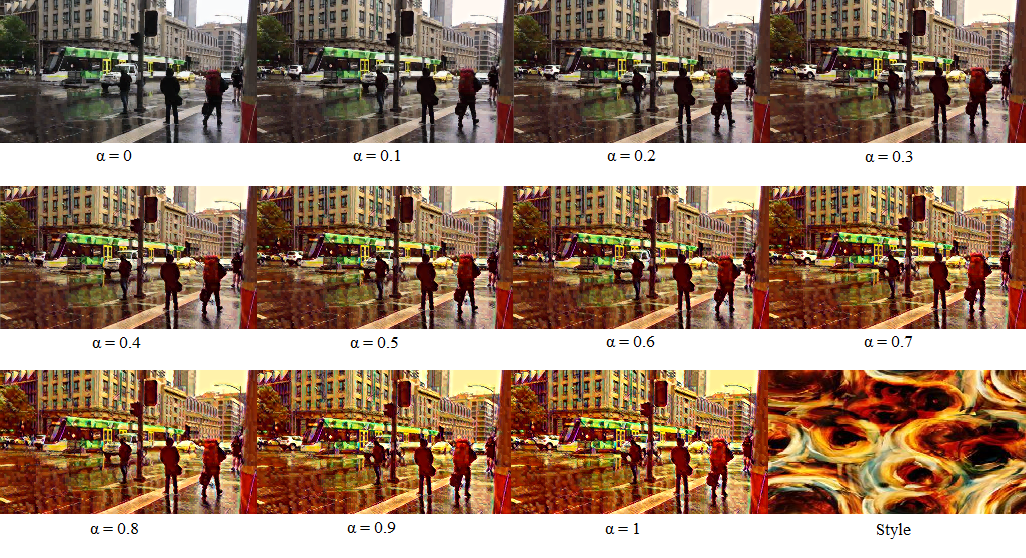
\includegraphics[scale=0.75]{Images/style1.png}
    \caption{Comparison between different values of style weight}
    \label{fig:style1}
\end{figure}

\subsection{Color preservation}
Style transfer give us a content image in style of the chosen, another image. To output has a all details like lighting, shapes and colors. Using method of color histogram matching we can preserve color of content image and then transfer the style. The key of this method is create new style $S'$ by changing colors of style picture to colors matching with content, and then use style transfer algorithm. \\
We are want each pixels $x=(R,G,B)$ to match mean and covariance of RGB values to new style, by using following transformation: $$x_s\rightarrow{}Ax_s+b$$ where A is a 3x3 matrix and b is a 3-vector. We choose A and b to satisfied by the constraints: $$b=\mu_C - A\mu_S$$ $$A\sum_SA^T = \sum_C$$ where $\mu_S$ and $\mu_C$ are mean colors of the style and content, $\sum_S$ and $\sum_C$ are pixel covariances. That give us family of solutions to A, now we use the Cholesky decomposiotion but it depends on colors channel ordering, or 3D color matching formulations, we choose this method. \\
The eigenvalue decomposition of a covariance matrix will be $\sum=UAU^T$, we can define matrix square-root as $\sum^{1/2}=UA^{1/2}U^T$, with this and the transformation is following by: $$$$

\subsection{Video stability}
One of goals for high-quality style transfer is stability. Let $F_1$ and $F_2$ be 
two video frames relatively close in time and $T$ a style transfer algorithm transforming
a single frame. We can define stability of $T$ by mean difference between
$| F_1 - F_2 |$ and $|T(F_1)-T(F_2)|$. The smaller that difference, the more stable $T$ is.
This definition says that if a certain region doesn't change between $F_1$ and $F_2$, then
it also shouldn't change between $T(F_1)$ and $T(F_2)$, that is the transformed video
shouldn't flicker too much. Definition also implies changes in orgiginal video
should be reflected in the stylized video, but it's an obvoiys requirement and it's
the former property that we usually call stability.
Stability can be expilicitly guaranteed by use of special loss functions
and proper training procedure \cite{stability1, stability2}. The model we base our work
on however learns stability by design \cite{Li2018}, so there is no need for
any auxillary techniques. We examine to what extent network pruning damages this 
property. We conduct the experiment using a single style image and 3 videos with motionless
camera. Results are presented in Figure \ref{fig:heatmap}.
For each of $3\times3$ grids, the third row shows heatmaps of differences between 
two images above it. A hypothetic perfectly stable style transform algorithm would
produce the same heatmaps as the ones in left column. While both models perform
resaonbly well for second and third video, they completely fail in the first case.
The reason for such behaviour is progressive change of brightness of the sky
which can't be seen in shown frames. Sky's brightness changes significantlly 
as a result of some vehicle driving in front of camera. In other words
stylizing poorly recorded video results in instability and noise. Comparing
original and pruned model, we also see the latter is less stable for this video,
though stripes produced by original model may seem even worse than overall
noise outputed by pruned model. In the second case both networks perform equally well
and their heatmaps are only slightly more noisy than the original heatmap.
For the third video pruned model is only a bit more unstable than original model.
Overall pruning seems to reduce stablility only by a small margin provided original network
preserves stability. In situation where original network fails to do so, pruned model
magnifies errors though.
\begin{figure}[h!]
\centering
    \includegraphics[width=0.9\textwidth]{heatmap.jpg}
    \caption{Comparison of stability between original (middle column) and pruned
    (right column) model. Left column shows original video frames. For each of
    $3\times3$ grids first two rows show two frames close two each other
    ($1$ to $5$ frames of difference, depending on video's framerate) and the third
    row is heatmap of difference between them. To the right of the grid: used style
    image and heatmaps' scale.
    }
    \label{fig:heatmap}
\end{figure} 



\subsection{Style and content encoding} \label{two_encoders}
As mentioned in section \ref{network} the encoder had to be copied due to pruning
constraints. Since two resulting encoders were pruned and fine-tuned separately 
their sets of weights are different. In this section we shortly examine effects
of using wrong combinations of encoder in pruned model. Results for four possible combinations
of encoders are presented in Figure \ref{fig:mosaic_asym}.

        \begin{figure}[h!]
        \centering
            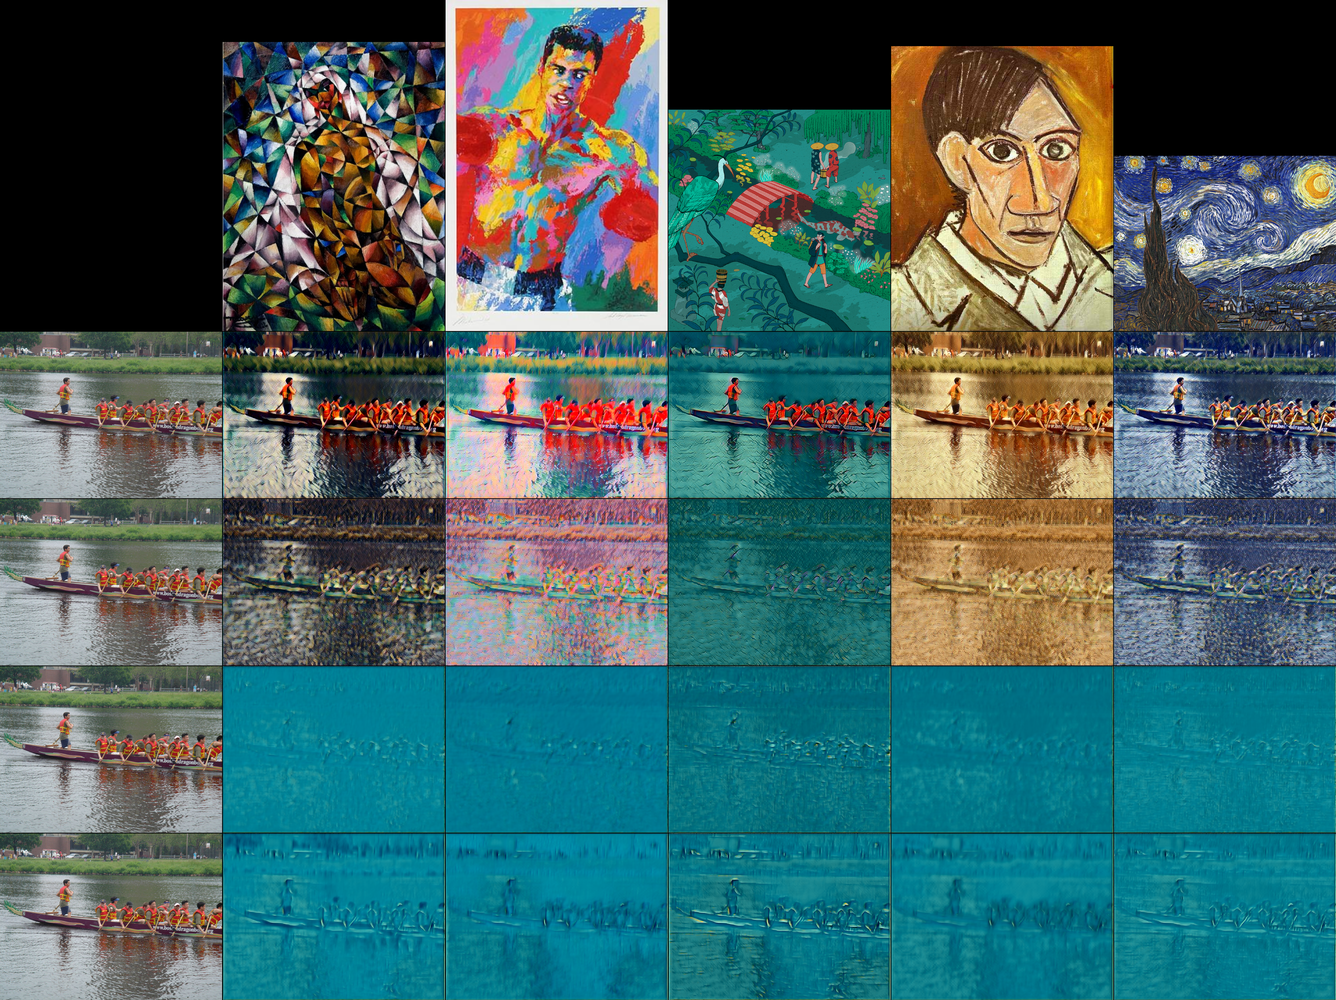
\includegraphics[width=1\textwidth]{mosaic_asym.png}
            \caption{Comparison of various configurations of network with respect
            to encoder used for encoding style/content image. From top to bottom:
            $S_E(S_I)$ and $C_E(C_I)$, $S_E(S_I)$ and $S_E(C_I)$,
            $C_E(S_I)$ and $S_E(C_I)$, $C_E(S_I)$ and $C_E(C_I)$, where
            $S_E$ and $S_C$ are style and content encoders, $S_I$ and $C_I$ are 
            style and content images.
            }
            \label{fig:mosaic_asym}
        \end{figure}
        
The first row presents default variant with proper configuration. 
We see that while style encoder $S_E$ is able to encode content features to some
degree (2nd row), content encoder $C_E$ fails completely at style extraction
(3rd and 4th row). This is expected, since $C_E$ can usually safely
discard most of color information in content image. On the other hand, $S_E$
should pay attention to both color and shapes. Consequently images in second row
are of a lot worse quality than first row, but content and style are still readily
recognizable. Comparing 3rd and 4th row, we see content 
is reconstructed better in the latter one. Again, this should be the case,
since content is encoded with $S_E$ in 3rd row and with $C_E$ in 4th row -
$C_E$ produces more accurate shape encoding than $S_E$ so images in 4th row are
sharper and less blurry.





\biblio % Needed for referencing to working when compiling individual subfiles - Do not remove
\end{document}
